\documentclass[../Main.tex]{subfiles}

\begin{document}

Because parts of this project were as much a learning exercise as an engineering one it took some experimenting with Windows Forms to build the proper mental model for how it all fits together, as a result writing unit tests was delayed until much later in development. This resulted in a design with numerous tight coupling issues between the model and the gui elements. 
Expanding the coverage of unit testing revealed many such issues, most (but not all) were resolved. 
There was a consistent issue with coupling the serializer class \textbf{Persistance} with the \textbf{Favourites} \& \textbf{History} classes, this was resolved in an unsatisfactory manner by creating a seperate static method to instantiate a testing version of these classes that are unlinked to the \textbf{Persistance} class.
The unit testing also presented issues when testing methods with async void signatures, resolving this issue would take a significant amount of refactoring and would mainly serve the purpose of making those methods unit testable. An unsuccessful attempt at testing such a case can be observed in Fig.~\ref{fig:TestCov} (right).

\begin{figure}[H]
    \begin{center}
        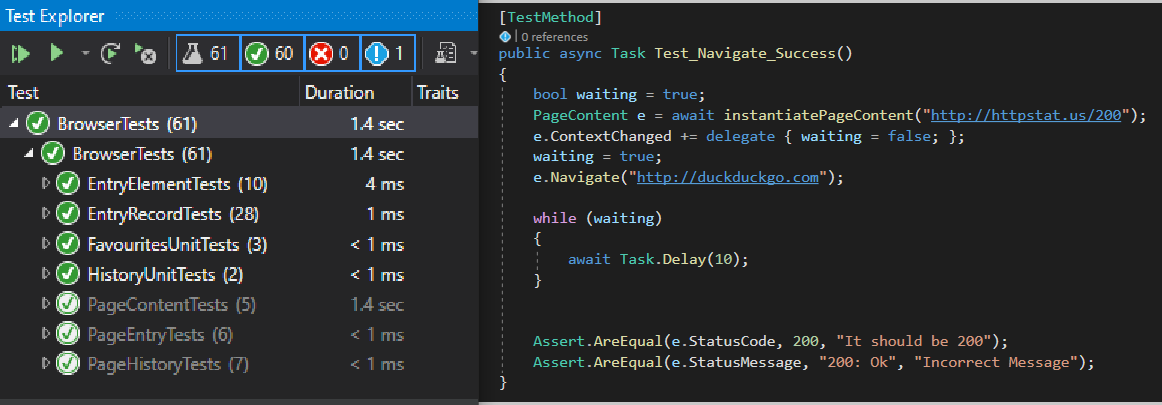
\includegraphics[width=1\textwidth]{TestCovBadTest.png}
    \end{center}
    \caption{(Left) Summary of the number of tests for each class. (Right) Unsuccessful attempt at testing async void method}
    \label{fig:TestCov}
\end{figure}

The classes related to the history/favourite do have excellent test coverage (aside from interactions with \textbf{Persistance}), these classes were mostly engineered in a loosely coupled manner and as a result it was quite easy to write tests for them. On the other hand the \textbf{PageContent} class has many async void methods, so the test coverage is poor.

Throughout development manual integration tests were performed, these were adequte at the beginning but as the code base grew the need for a more formal testing suite was becomming increasingly apparent. Ultimately the project had 61 unit tests to complement the regular integration tests.

\end{document}
